%%%%%%%%%%%%%%%%%%%%%%%%%%%%%%%%%%%%%%%%
%%%%% DATASET DESCRIPTION AND ANALYSIS
%%%%%%%%%%%%%%%%%%%%%%%%%%%%%%%%%%%%%%%%
\section{DATASET DESCRIPTION AND ANALYSIS}
The discussion in this section covers the datasets that were used for obtaining the training data, how the training data used in our research was selected from these datasets, and the preprocessing methods used before feeding the data into the neural network. 

%%%%%%%%%%%%%%%%%%%%%%%%%%%%%%%%%%%%%%%%
%%%%% DATASETS USED
%%%%%%%%%%%%%%%%%%%%%%%%%%%%%%%%%%%%%%%%
    \subsection{DATASETS USED}
        \begin{figure}[H]
            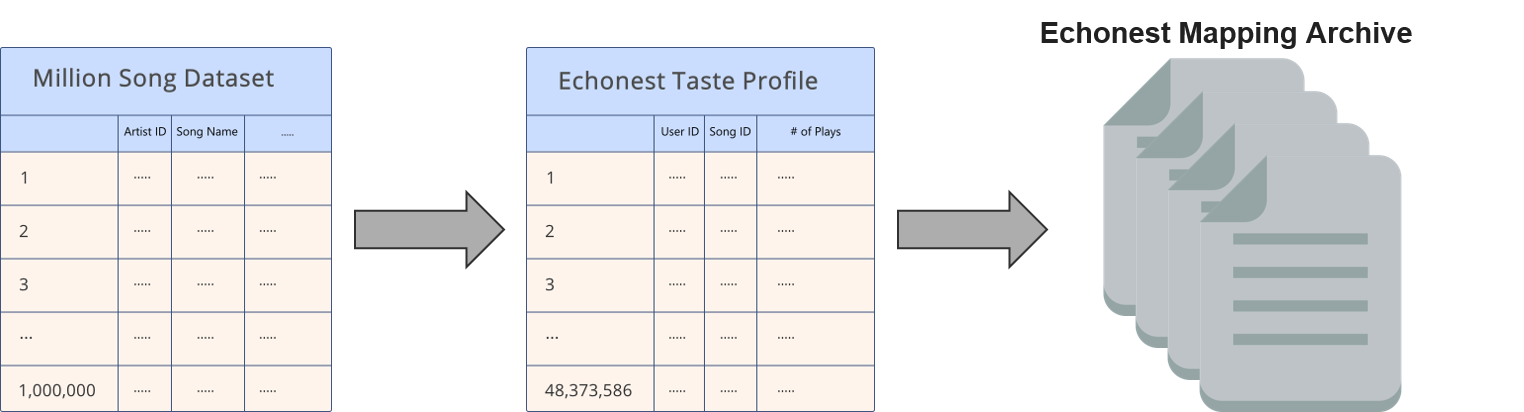
\includegraphics[width=0.45\textwidth]{dataset_mapping.png}
            \caption{Simple Graphic Displaying Datasets}
            \label{fig:datasets}
        \end{figure}

        \subsubsection{Million Song Dataset}
            The Million Song Dataset (depicted on the left in Figure \ref{fig:datasets}) is a dataset containing various fields of metadata for popular songs. \cite{msd_site} The data includes information such as the song title, artist name, album title, as well as more in depth information like the tempo of the song (BPM) and the estimated musical key that the song is played in. Many other researchers have used this dataset and it's subsets to perform music recommendation related research. \cite{Wang2014,Wang:2014:ICH:2647868.2654940,NIPS2013_5004} Unfortunately, all of the data provided by the subset is unusable for the purposes of the experiments performed here as no real-world user data is provided. However The EchoNest Taste Profile Subset provides this information and will be discussed next.
        \subsubsection{The EchoNest Taste Profile Subset}
        The EchoNest Taste Profile Subset (depicted int the center of Figure \ref{fig:datasets}) provides play count information using 384,546 songs of the Million Song Dataset for 1,019,318 prior EchoNest users. \cite{etp_site} There is a total of 48,373,586 records that contain the EchoNest song ID, the user ID of the user playing that song and the number of times that user played a song. This information is immensely useful for researchers that wish to perform a music recommendation analysis, or in our case, estimate how many times a user is likely to play a given song. 
        
        With the limited ability of real-world user data that is readily available via APIs due to permissions needed to access a user's information on popular music services, this archive is very valuable for research. For example, Spotify's API requires explicit permission for a user to simply read a user's recently played and top played tracks. \cite{spotify_permissions} Even then, these API queries are limited to 50 songs maximum, and are not guaranteed to not contain duplicates. \cite{spotify_recent,spotify_top} 
        \subsubsection{Echonest Mapping Archive}
        Due to the acquisition of The EchoNest by Spotify and it's subsequent shutdown, it is no longer possible to easily map the songs available in The EchoNest Taste Profile Subset or Million Song Dataset to other music services as this functionality was removed. However, a group of researchers created the The EchoNest Mapping Archive (depicted on the right in Figure \ref{fig:datasets}) that maps the songs includen in the Million Song Dataset to many other music services such such as Spotify, 7-Digital, MusiXMatch, and others in an archive of individual JSON files. \cite{map_site} Without this dataset, the only way to map between services would be by querying using Artist and Song names which is not guaranteed to provide accurate results. It is worth noting that the archive is not 100\% complete. In our experiments, we were able to obtain between 40\% and 60\% of the Spotify IDs for songs we obtained during data extraction.
        
%%%%%%%%%%%%%%%%%%%%%%%%%%%%%%%%%%%%%%%%
%%%%% TRAINING DATA EXTRACTION
%%%%%%%%%%%%%%%%%%%%%%%%%%%%%%%%%%%%%%%%
    \subsection{TRAINING DATA EXTRACTION}
    The final set of data that was used for training and evaluating our network models was obtained primarily from The EchoNest Taste Profile Subset and secondarily from The EchoNest Mapping Archive. The triplets from The EchoNest Taste Profile Subset were loaded into a MySQL database and results were obtained after various queries narrowing down the dataset to an acceptable level based on alloted computation time and storage space. These queries are explained in the below subsections. Once the final records were obtained, The EchoNest Mapping Archive JSONs were queried to obtain the corresponding Spotify IDs, added to a Spotify Playlist using the Spotify API and music data was obtained using a Spotify Premium Membership.
        \subsubsection{Limiting Maximum Number of Plays}
        After initially examining the dataset, it appeared that there were quite a few outliers due to some play counts. Some records showed over 1000 plays for a single user/song pair, so it was decided to trim outliers from the dataset by limiting the maximum number of plays per record to 200 plays. In total this trimmed the entire dataset from approximately 48 million records down to 48,370,466.
        \subsubsection{Obtaining the Top 5 Users}
        From the trimmed dataset, the top 5 users were selected based on the total aggregate number of plays. These were obtained using an SQL query to sum the number of plays, grouped by User ID. The decision to choose the top 5 users was done in order to be able to provide a comparison of network structures for multiple users and to see whether or not a model exists that performs universally acceptably. The decision to only perform network training on the data for 5 users was due again to limited training time and storage budgets.
        \subsubsection{Choosing Training Data}
        The final data set used for training the networks was obtained by querying the database for all songs listened to by at least two of the top 5 users. This resulted in a total of 341 songs, of which only 150 had corresponding Spotify IDs in The EchoNest Mapping Archive JSON files. These Spotify IDs were then added to a Spotify Playlist and the audio files were downloaded using a Spotify Premium Membership.
        
%%%%%%%%%%%%%%%%%%%%%%%%%%%%%%%%%%%%%%%%
%%%%% DATA PREPARATION
%%%%%%%%%%%%%%%%%%%%%%%%%%%%%%%%%%%%%%%%
    \subsection{DATA PREPARATION}
    This subsection describes how the user and audio data were treated during the training process and the preprocessing methods used before feeding in the data to the network.
        \subsubsection{User Play Information}
        Of the 341 final songs selected, a CSV file was generated for each user containing the records for that User ID with each record consisting of the User ID, Song EchoNest ID, and number of plays. In order to be able to compare the performance per user directly, the column of user plays was standardized for each user before being used as training data by the network. The function in Algorithm \ref{alg:load-userdata} was implemented for loading and preprocessing the user data. 
        \begin{algorithm}[h]
            \KwIn{Location of User Data, Location of Music Data}
            \KwOut{Tuples of (User ID, Song ID, Standardized Play Value)}
            \SetKwProg{function}{load\_and\_preprocess\_user\_data}{end}
            \function{
                $userData$ = read user record CSV file\\
                $musicAvailable$ = list songs in music directory\\
                \ForAll{song $s$ in $userData$}{
                 \If{ Song $s$ is not in $musicAvailable$}{
                      Remove $s$ from $userData$
                  }
                 }
                 Standardize number-of-plays column in userData\\
                 \Return userData
            }
        \caption{Load and Standardize User Data}
        \label{alg:load-userdata}
        \end{algorithm}

        \subsubsection{Audio Data}
        In order to make the network compatible with songs of varying length as well as make recommendations based on partial song information, the input to the network was limited to 5 second song clips. As will be explained in Section \ref{sec:nn-models}, the number of these 5 second vectors consumed by the network varied based on the network architecture, however each individual clip was no longer than 5 seconds. In order to process the audio files, two domain-specific Python libraries were employed: PyDub and LibROSA. \cite{librosa-site,pydub-site} In this case, PyDub was used to split the songs into their 5 second increments (depicted in figure \ref{fig:audio-split}) and LibROSA was used to convert the split MP3 files into NumPy arrays.
        \begin{figure}[H]
            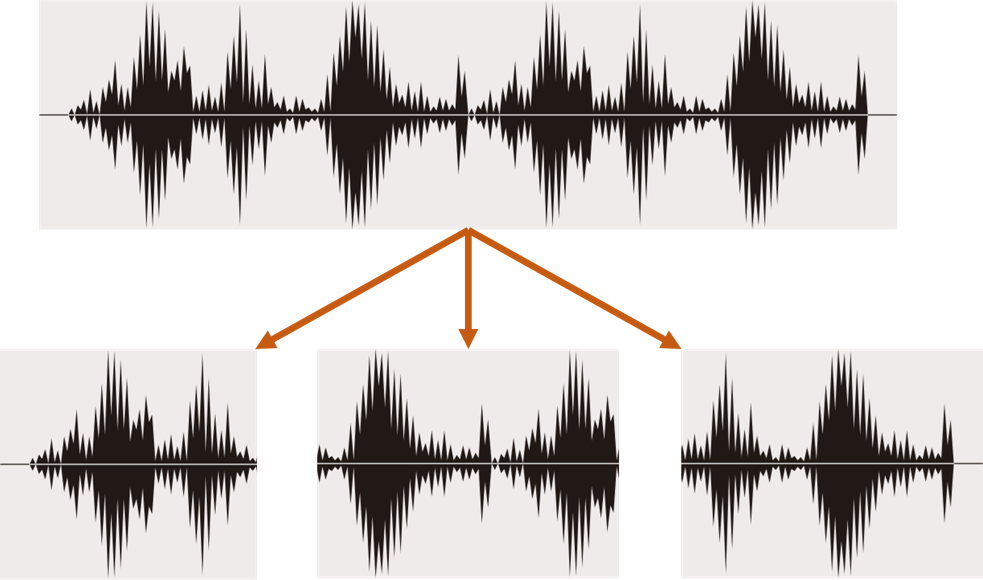
\includegraphics[width=0.45\textwidth]{song_split.png}
              \caption{Figure Depicting Audio Split}
              \label{fig:audio-split}
        \end{figure}
